\chapter{材料与方法}\label{chap:Material_approach}
%With speculative execution, it calculates memory addresses and initiates cache refills early
\section{相关工作与材料}\label{sec:meterial}
	前有经典的Alpha 21264和MIPS R10000成熟产品,后有开源的RISC-V BOOM处理器设计,都是非常优秀的相关工作。而它们的设计报告文献作为宝贵的材料同样值得参考与借鉴。吸收它们的优秀结构设计并灵活运用到自己的处理器设计当中。
	\subsection{Alpha 21264}\label{subsec:alpha}
	
	Alpha 21264是处理器设计历史上高性能的代表之作。下面从\textit{THE ALPHA 21264 MICROPROCESSOR}\citep{Alpha21264}这篇技术报告分析Alpha 21264的微结构设计。
	
	首先Alpha 21264整体的流水级模块级框图\ref{fig:alpha_stage}一共切分成了7个大的阶段。
	\begin{figure}[!htbp]
		\centering
		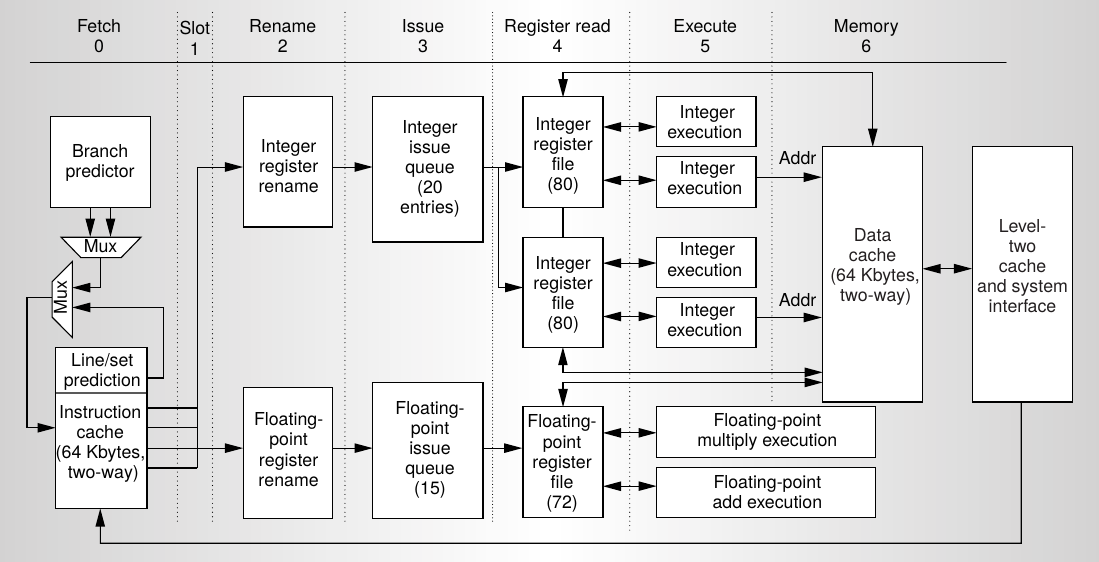
\includegraphics[width=0.8\linewidth]{21264}
		\bicaption{Alpha 21264流水线阶段。\citep{Alpha21264}图 2.}{Stages of the Alpha 21264 instruction pipeline. Figure 2 of \citep{Alpha21264}.}
		\label{fig:alpha_stage}
	\end{figure}
	
	从第0级的取指开始往流水线的下游方向逐级分析一些设计的亮点。
	\begin{enumerate}[label=(\alph*)]
		\item \textbf{取指}。21264为了提高取指的效率,着重强调了两个设计,一是icache的行和路预测,二是分支跳转预测。
		
		由于21264的icache采用的是两路组相连,一种方案是把行对应的两个路都读出来,然后在做二选一逻辑,不过这样电路延迟就增加了,而且可拓展性也不好,到四路的延迟更大。所以21264选择了另外一种方案 --- 路预测,采用和分支预测相似的两位饱和计数的技术,对于大多数程序而言正确率都能达到85\%$ \sim $100\%,猜得准的同时猜错代价很小,绝大多数情况下只有1个周期\citep{Alpha21264}损失。所以采用路预测对电路主频的提高收益大于损失的周期数。
		
		与icache路预测情况不同,21264最多容纳80条指令乱序执行,转移指令猜错代价很大。所以分支预测就成为了提高21264效率非常重要的一环。为了追求预测的正确率,21264实现了复杂的锦标赛预测方案,动态的选择两种类型的分支预测器的预测结果 --- 一是用跳转指令本身的跳转历史,二是用全局的跳转历史。预测准确率比采用更大的表独立各采用上述两种方案更好,达到90\%$ \sim $100\%\citep{Alpha21264}。具体来看,21264一共维护了3个表,结构如图\ref{fig:branch_21264}所示。
		\begin{itemize}
			\item 一张局部历史表,能够存放1024条指令10 bits的自身跳转历史,面积$ 1024\times 10 $ bits.
			\item 一张全局预测表,配以一个12 bits的全局历史,所以有4096项,每一项是2位饱和计数器,面积$ 4096\times 2 $ bits.
			\item 一张选择表,用来选择两种预测机制中更好的一个,和全局预测表一致,共有4096项,也采用两位饱和计数器,面积$ 4096\times 2 $ bits.
		\end{itemize}
		\begin{figure}[!htbp]
			\centering
			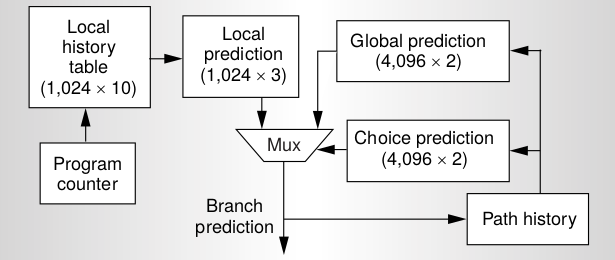
\includegraphics[width=0.7\linewidth]{branch}
			\bicaption{21264锦标赛分支预测框图。\citep{Alpha21264}图 4.}{Block diagram of the 21264 tournament branch predictor. Figure 4 of \citep{Alpha21264}.}
			\label{fig:branch_21264}
		\end{figure}
		\item \textbf{重命名与乱序发射}。在21264的设计中,乱序的部分为了效率考虑,采用主频更高的时钟域。
		
		一个周期最多能够取回4条指令,先锁存一个周期,然后在CAM形式的重命名表中进行重命名和寄存器的分配。需要注意的是,和MIPS一样,Alpha在重命名阶段要特殊处理条件移动指令的映射关系。重命名完毕消除了写后写和读后写的冲突,但是依旧保留了写后读冲突。之后将指令写入发射队列中。发射队列采用分离式,分为整数指令队列和浮点指令队列,最多可以动态发射出6条指令,四条整数指令,两条浮点指令。使用记分牌来判断指令的操作数是否准备就绪。发射的细节上,微结构上有一个20项的定点队列和一个15项的浮点队列,队列只发射的是那些操作数都已经准备好的指令。与此同时,队列由仲裁器来决定填入新的指令。上述模块的逻辑可以由图\ref{fig:rename_21264}来直观的描述。
		\begin{figure}[!htbp]
			\centering
			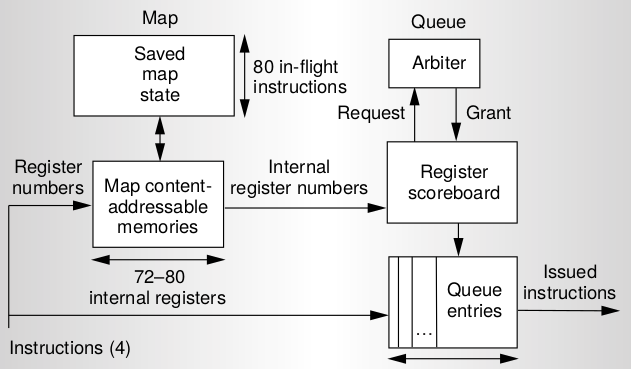
\includegraphics[width=0.6\linewidth]{rename}
			\bicaption{21264寄存器重命名以及出入队列阶段框图\citep{Alpha21264}图 5.}{Block diagram of the 21264’s map (register rename) and queue
				stages. The map stage renames programmer-visible register numbers to
				internal register numbers. The queue stage stores instructions until they
				are ready to issue. These structures are duplicated for integer and floating-
				point execution. Figure 4 of \citep{Alpha21264}.}
			\label{fig:rename_21264}
		\end{figure}
		上图中有一个Saved map state模块,非常重要,它的作用是转移预测错误的恢复处理器状态。注意该表有80项,也即每一条指令分配一项,这样处理器可以从任何一条指令之后精确地恢复状态,而不会受到跳转指令数量的约束。但是缺点是非常消耗资源。当然不光是转移预测错误的恢复,例外中断的状态恢复同样也是用这个表的,但和分支预测错误的恢复机制略有不同。
		\item \textbf{乱序执行引擎}。由于发射队列每一周期能够发射6条指令,所以引擎一共有6条执行流水线。
		
		21264具有特色地将整数寄存器堆分裂为两个集群,均有重复的80项。对应的属于整数的4条流水线被均等的分配到了两个集群下。虽然这样增加了集群之间互相广播的电路延迟和周期数,但是却使得设计更加简单快速。最根本的原因是减少寄存器堆的读端口数目。如果不分为两个集群,每条指令需要两个操作数一共就需要8个读端口,加上寄存器堆有80项,物理布局布线之后的时序非常的差,远远不如只有4个读端口的情况。Alpha这个用空间换时间的做法也是无奈之举。这也给后来的设计者一种警示,为了处理器的主频,必须要控制寄存器堆的读端口数量。
		\item \textbf{指令的提交与退出}。指令是按照次序提交退出的。
		
		在21264设计文档中给出最为有用的信息是每一条指令都要带着之前旧的目的物理寄存器号,并在顺序提交退出后回收这个该物理寄存器。首先这个机制能够维护有远远不断的物理寄存器可以再生分配,其次说明了这个机制有正确性的保障。所以毕业设计中的做法和Alpha的做法保持一致。

		\item \textbf{内部访存部件设计}。
		
		为了降低访存的平均延迟,Alpha 21264在访存上做了很多不惜成本的设计,将性能做得非常强悍。主要体现在:一个周期能够执行两条乱序的访存请求,也即首先dcache即必须是双端口的;访存系统能够同时追踪32条in-flight的store指令,32条in-flight的load指令和8条in-flight的指令或者数据cache miss;dcache是64KB,2路组相连的结构\citep{Alpha21264}。处理器内部访存控制结构采用经典的load queue(LDQ)和store queue(STQ)数据结构。每个队列均有32项和上述可以同时追踪的load/store指令数量一致\citep{Alpha21264}。毕业设计中基本的设计参考的就是21264的设计,但是做了一些面积功耗的优化与改进。
		\item \textbf{内部memory系统}。21264设计了高带宽和低延迟的memory系统。
		
		这篇设计文档最后花了较多的篇幅来介绍,包括cache预取,填入和替换策略以及总线的介绍,以及用8项的miss address file (MAF)来同时追踪上文提到的8条in-flght cache miss访存请求的机制。内部memory系统是非常复杂的一个领域,在毕业设计中出于简化的考虑不会继续做深入的分析和设计。
	\end{enumerate}
	
	\subsection{MIPS R10000}\label{subsec:r10000}
	
	R10000是一款四发射乱序处理器,执行引擎有五个流水线;为了隐藏访存延迟,R10000用了两级均为两路组相连写回的cache,并且是非阻塞式的,也即一个cache行的miss不会阻塞另外cache行的访问;在处理器内部in-flight的指令数最多有32条\citep{MIPS1996}。处理器的整体设计参见模块框图\ref{fig:r10000_block},流水线(图\ref{fig:r10000_pipeline})级数的编号是从1开始的。
	\begin{enumerate}
		\item 第一级发出取指请求,并对齐下一周期的四条指令。
		\item 第二级对取回的指令做译码然后进行重命名,同时计算跳转分支指令的目的地址反馈到取指单元.
		\item 第三级将重命名完的指令写入发射队列中,直到操作数都已经准备好,才能从队列中发射出来。在后半个周期的时候读寄存器堆获取源操作数。
		\item 第四级开始执行,整数指令需要一个周期,load指令需要两个周期,浮点指令需要三个周期,
		\item 写回是在得到结果后一个周期的前半个周期。
	\end{enumerate}
	\begin{figure}[!htbp]
	\centering
	\begin{subfigure}[b]{0.7\textwidth}
		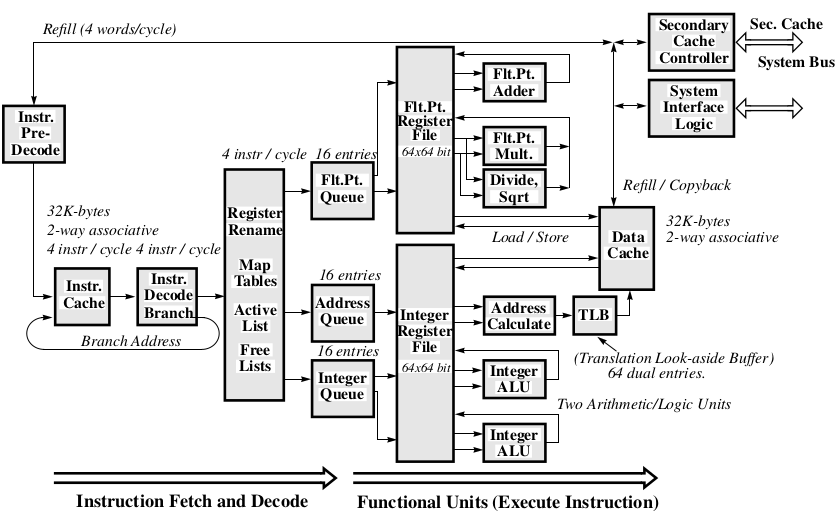
\includegraphics[width=\textwidth]{r10000_block}
		\caption{}
		\label{fig:r10000_block}
	\end{subfigure}
	\begin{subfigure}[b]{0.7\textwidth}
		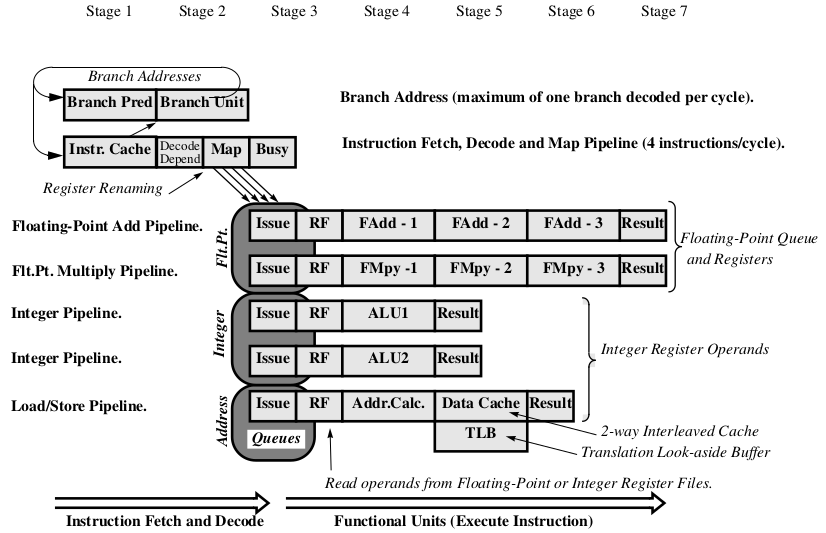
\includegraphics[width=\textwidth]{r10000_pipeline}
		\caption{}
		\label{fig:r10000_pipeline}
	\end{subfigure}
	\bicaption{MIPS R10000整体设计。\citep{MIPS1995}图2和3. (a) R10000模块框图,(b) R1000流水线。}{MIPS R10000 overall design. Figure 2 and 3 of \citep{MIPS1995} (a) R10000 Block Diagram, (b) R10000 Pipelines.}
	\label{fig:r10000_total}
	\end{figure}

	与Alpha 21264相似之处在于对整数指令和浮点指令采用了分离式的处理方案。但是与Alpha 21264相比,性能却差了很多。这与微结构的设计是分不开的。仅仅是通过观察两者的整体设计图以及一些最基本的参数,不考虑转移预测率和访存的性能,都不难找到R10000与21264之间差距的几点原因:
	\begin{enumerate}[label=(\alph*)]
		\item 因为都是采用分离式结构,只需对比整数指令。R10000最多支持32条in-flight的指令乱序调度,但是21264却支持80条,是R10000的两倍多,所以对指令的并行性有更大程度的挖掘。还有一点是,由于两者超标量宽度同样是4,但是由于R10000允许的in-flight指令比21264少太多,很容易导致发射队列塞满而阻塞取指部件供应指令。
		\item 流水级的切分不合理,导致时序太差。如果用统一的从1开始编号,那么意味着21264是在第5个周期读寄存器堆的,而R10000在第3个周期就要读取了。足足提前了两个周期,换言之,R10000将21264五个周期的工作压缩到3个周期,电路时序之差就可想而知了。有两点特别突出:第一,从icache同步读回的指令,组合逻辑就要做译码,重命名,算跳转地址,所以第二级的电路延迟非常大;第二,第三级中要先从16项的队列中选出发射的最多可以有两项(定点队列),然后组合逻辑去读寄存器堆,这一级的时序也是非常紧张。
		这两点Alpha 21264都分别用两个周期来做的,所以R10000少的两周期就是这么来的。
		\item 在21264中已经面对的问题 --- 对于寄存器堆的读端口要控制。为此21264还专门做了两份重复的寄存器堆来缩减读端口。如果看配置,21264是80项,有4个读端口;而MIPS则是64项,有6个读端口。因为读端口多了两个,所以单就寄存器堆的时序上,R10000就不如21264,更何况21264是用一整级来做读寄存器堆的逻辑的。
	\end{enumerate}
	
	综上所述,在21264主频已经达到500$ \sim $600MHz的时候,R10000主频只能做到200MHz;所以在SPEC95性能测试程序上,21264定点程序在30分以上,浮点程序在58分以上,而R10000定点程序峰值为9分,浮点程序的峰值为19分,是21264性能的1/3不到\citep{Alpha21264,MIPS1996}。 但这些并不影响R10000同样存在一些值得借鉴的设计思路,下面梳理一下R10000的一些设计亮点:
	\begin{enumerate}[label=(\alph*)]
		\item 取指部件。
		
		\citep{MIPS1996}提出的设计思路是处理器取回来的指令带宽上要高于执行部件,将队列填充满非常重要,这样基本上就能在每一个周期都找到可以被发射的指令。和一般取指需要取指宽度对齐不同,R10000虽然取指宽度是4字(1指令/字),但是可以在16字指令cache行中以任意字对齐,这样可以提高取值的效率。通过一个对cache读出放大器简单的修改,基本上是四选一的逻辑。同时,为了简化连续的取指的时序,当发射队列或者活跃表已经满时,指令会被先进入一个八字的指令缓存\citep{MIPS1996},也即最多可以缓存8条未被译码的指令。这一点已经借鉴到了自己的处理器设计当中,参见第3章节。
		\item 分支跳转单元。
		
		R10000在这一方面做的也没有21264性能高,体现在两个方面。第一,预测策略上,只有一个简单的有512项的两位饱和计数器,在Spec92整点程序中预测率也只有87\%\citep{MIPS1996}; 第二,设有分支栈,每当有译码到分支指令时,就会把处理器的状态压入栈中,作用是当分支预测错误处理器能够恢复到错误跳转前的状态。对比21264为每一个指令都存储对应的状态的做法,R10000显然会受限于高分支指令占比的程序以及程序片段。为了快速恢复,撤销掉分支预测错误后面的指令,R10000的每一条指令都带有4-bit的掩码,对应于分支栈,指示依赖于哪一项分支跳转。如果依赖该条分支指令,该位掩码置上。当分支预测错误就可以根据掩码的信息来撤销误取的指令。
		\item 寄存器重命名。
		
		见图\ref{fig:r10000_rename},不同于21264的CAM重命名表,R10000的重命名表是RAM的形式。考虑到HILO寄存器的存在,并且排除永远为$ 0 $的r0的寄存器,整数指令的重命名表是一张$ 33\times 6 $-bit的16读端口4写端口的RAM\citep{MIPS1996}。在重命名的相关控制逻辑上,R10000使用了三个数据结构 --- Free list, Active list和Busy-bit tables. 简言之,这三个数据结构的作用分别是:Free list负责记录更新未被使用的寄存器号用来进行物理寄存器的分配;Active list作用相当于Reorder buffer,记录在处理其中in-flight的活跃指令;Busy-bit tables用来指示当前物理寄存器中的值是否有效。
		\begin{figure}[!htbp]
			\centering
			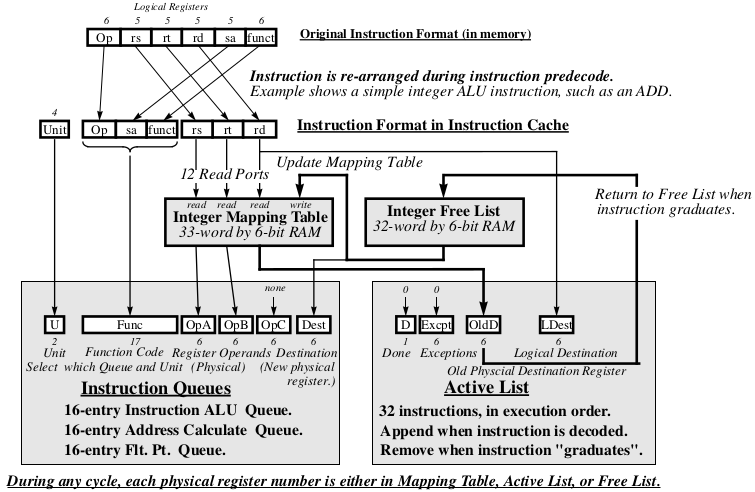
\includegraphics[width=0.7\linewidth]{r10000_rename}
			\bicaption{R10000寄存器重命名机制图解。\citep{MIPS1995}图4.}{Register Renaming of MIPS R10000. Figure 4 of \citep{MIPS1995}.}
			\label{fig:r10000_rename}
		\end{figure}
		
		\item 发射队列。
		
		除了常规的定点队列和浮点队列外,R10000还增加了一个地址队列,也可以被称为访存指令队列。为循环队列的形式,有16项。但这也不是新奇的设计,功能上和21264中的LDQ和STQ设计类似,只是将load和store指令统一存放在一起而已。
		\item 其他方面如运算单元的设计和内存层级结构并不在毕业设计范围之内,所以不做探讨。
	\end{enumerate}

	\subsection{RISC-V BOOM}\label{subsec:BOOM}
	
	BOOM是伯克利分校为了向学术界和工业界推广RISC-V ISA而设计出来的乱序处理器,其全称为The Berkeley Out-of-Order Machine。首先BOOM是伯克利分校在校的博士生们设计的,主要参考的是之前提到的两款经典的处理器Alpha 21264和MIPS R10000. 采用Chisel语言来编写,而且由于不是采用和21264、R10000类似的定制电路,诸如队列的项数,cache的大小,甚至发射指令数量都是参数化可配置的,所以强调参数的具体数字是没有多大意义的。但是像超标量宽度为2的参数基本上是固定的,也即BOOM的取指单元每一拍取回两条指令。
	
	BOOM经历了先后两代的演化,从版本1(BOOMv1)到版本2(BOOMv2)的变化能够十分真切的看出其在微结构上的瓶颈、改进重点和设计权衡。
	
	BOOMv1在流水级的切分参考了R10000,分成了六级 --- 取指、译码/重命名、发射/读寄存器、执行、访存、写回\citep{Celio:EECS-2017-157}。这种流水线的切分方案在MIPS R10000章节\ref{subsec:r10000}已经分析过是极不合理的,电路主频做不好。而且BOOMv1的整数寄存器和浮点寄存器是统一的,这样导致的后果是寄存器的项数和读端口数量(共有7个读端口和3个写端口)都很多;另外,BOOMv1采用了统一的发射队列,发射指令数量为3,也即在同一个队列里要一个周期要选出3条准备就绪的指令发射\citep{Celio:EECS-2017-157}。这样的设置同样极不合理,综合得到的电路变得异常复杂,时序会异常不好。综上,虽然IPC的比较上BOOMv1比BOOMv好了20\%\citep{Celio:EECS-2017-157},但是BOOMv1微结构设计糟糕,参考意义不大。下面着重来分析BOOMv2的值得借鉴的微结构设计:
	\begin{figure}[!htbp]
	\centering
		\begin{subfigure}[b]{.45\textwidth}
			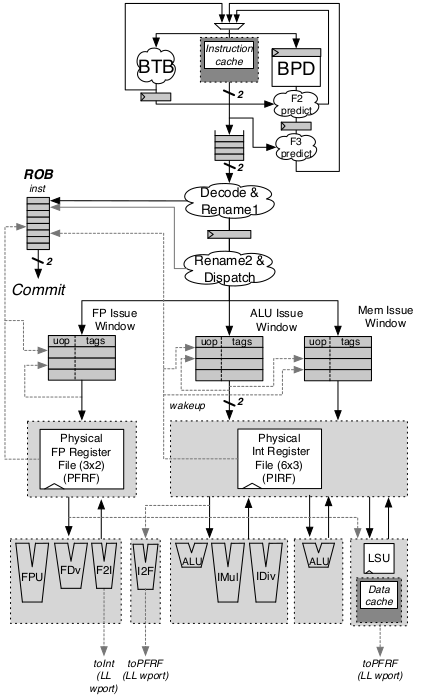
\includegraphics[width=\textwidth,height=12cm]{boomv2_tot}
			\caption{}
			\label{fig:boom_total}
		\end{subfigure}\qquad
		\begin{subfigure}[b]{.45\textwidth}
			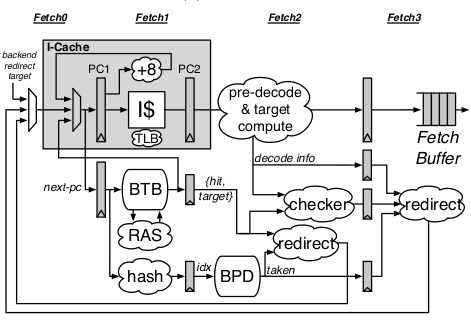
\includegraphics[width=\textwidth,height=5.5cm]{boom_ftend}
			\caption{}
			\label{fig:boom_ftend}
			
			\vspace{2ex}
			
			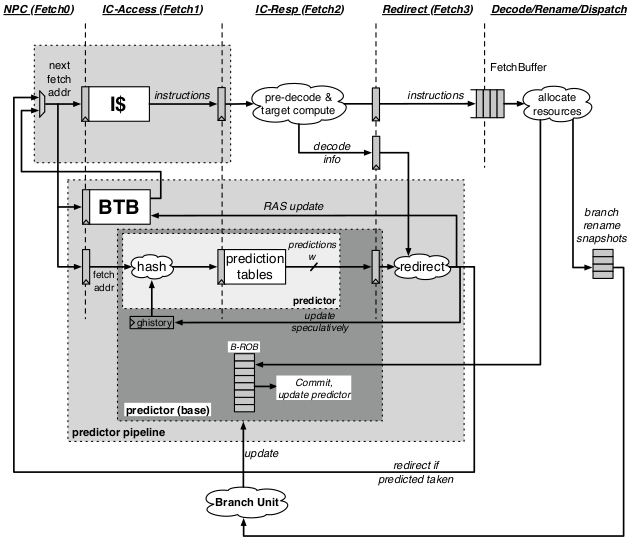
\includegraphics[width=\textwidth,height=5.5cm]{branch_fig_4_3}
			\caption{}
			\label{fig:boom_predictor}
		\end{subfigure}
		\bicaption{BOOMv2的全局设计以及前端设计图。\citep{Celio:EECS-2017-157}图2(b)和3(b), \cite{Celio:EECS-2018-151}图4.3. (a)BOOMv2的全局设计。(b)前端设计图。 (c)前端细节设计图。}{BOOMv2 overview and Frontend design. Figure 2(b) and 3(b) of \citep{Celio:EECS-2017-157}, Figure 4.3 of \cite{Celio:EECS-2018-151}. (a)BOOMv2 overview, (b)Frontend design, (c)Frontend design with more details.}
		\label{fig:boomv2}
	\end{figure}

	\begin{enumerate}[label=(\alph*)]
		\item 前端的设计。
		
		在BOOM相关的论文\citep{Celio:EECS-2017-157,Celio:EECS-2018-151}中,强调了前后端的概念。事实上,这是一个非常优秀的理念,很值得借鉴到自主的处理器设计之中。前端负责项后端供应指令,连续不断的指令流的供应就显得尤为重要。为了预测率并且权衡面积、关键路径延迟和预测错误流水线的取消开销等多方面的考虑,在BOOMv2的前端中,加入了多种不同的转移预测技术。
		
		\textbf{跳转目标缓存(BTB)},结构如图\ref{fig:BTB}存储了一定数量的指令地址(PCs)到跳转目标的映射集合。处理器用PC当做索引,以CAM的方式进行查找,如果命中,则重定向指令流从跳转目标开始重新取指。对于分支指令,另外借助饱和计数器来进行跳或不跳的预测。为了面积和时序的优化,可以用比如20-bit的PC低位的部分来代替整个32位或者64位的PC\citep{Celio:EECS-2017-157},这样对预测率几乎没有任何影响。
		\begin{figure}[!htbp]
			\centering
			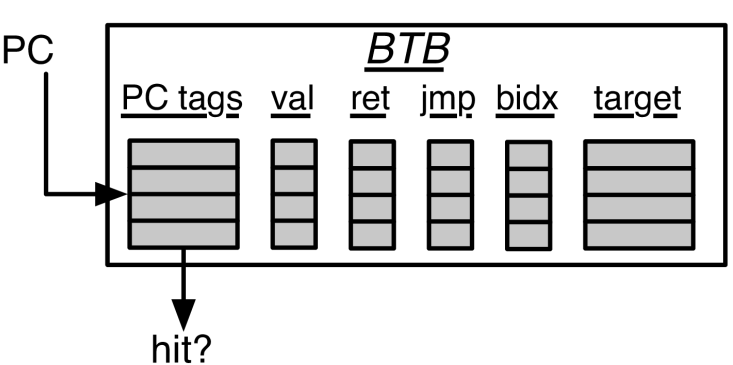
\includegraphics[width=0.5\linewidth]{BTB}
			\bicaption{BTB结构示意图。\citep{BOOMDoc2018}图3.2.}{BTB Unit Structure. Figure 3.2 of \citep{BOOMDoc2018}.}
			\label{fig:BTB}
		\end{figure}
	
		\textbf{返回地址栈(RAS)},用来预测函数调用的返回。寄存器类的跳转指令非常难以预测,因为寄存器的值是不固定的。函数调用后返回的地址虽然也是从寄存器读取的,但是却极具规律性,就等于调用该函数的指令的PC值加4,因此很好预测。而且函数的调用可以用栈来完全的刻画,所以预测器只需检测到函数调用的时候把调用函数的指令$ PC+4 $就压入栈中,等检测到函数返回的时候再弹出栈,就能很好的预测对绝大多数函数调用的情况。
		
		\textbf{分支预测器(BPD)},专门针对分支指令的优化,每一项只存储两位饱和计数器来预测跳或者不跳的跳转方向,所以必须要在知道是跳转指令以及跳转指令结果的情况下才能使用。这样,BPD可以和BTB一起并行查找,当BTB得到跳转地址以及是否命中的信息的时候,BPD刚好能够得到跳转的方向;或者BPD等到指令取回开始译码并算得目标地址的时候给出跳转方向。由于每一项的位数很小只有两位,所以项数可以做的很大,如1024项。这样就可以配合着10-bit的全局跳转历史通过哈希算法如gshare得到对于BPD的索引号索引BPD表得到跳转方向的信息。
		
		见图\ref{fig:boom_ftend},展示了前端各个预测单元的交互方式和流水线的组织形式。可以看到指令在F2阶段取回,被译码并计算得到目标地址,然后在F3阶段给出指令重定向的信息。这样能够给哈希算法整整一个周期的时间计算。BTB的组织形式可以是多样的,比如参考cache的设计采用多路组相连的形式而不一定要采用全相连的形式,这样可以节约电路的时序。
		
		还有一个模块值得注意的是在图\ref{fig:boom_predictor}中最灰方框中展现的名为B-ROB的单元,这一是个只存放分支跳转指令的小型的重排序缓存,里面保存了非常重要的处理器状态的快照(Snapshot),用来在分支预测错误时候对处理器的状态进行恢复,这同样参考的是MIPS R10000。
		\item 重命名阶段的数据结构和操作都很大程度借鉴了MIPS R10000的做法,不做赘述。
		\item BOOMv2的发射队列采用了和MIPS R10000几乎相同的组织形式,一个16项的定点指令队列,一个16项的浮点指令队列和一个16项的访存指令队列,见图\ref{fig:boom_total}。采用的是移位队列的形式(collapsing queue)并采用级联的优先编码器(cascading priority encoder)去选择最早就绪的指令发射出去\citep{Celio:EECS-2017-157}。不过BOOM是可配置的,所以BOOM同样提供了另外一种R10000风格的无严格先后次序的发射,但这样会导致性能不佳。
		\item 访存单元。BOOM设计了3个队列,the Load Address Queue (LAQ), the Store Address Queue (SAQ), and the Store Data Queue (SDQ)\citep{BOOMDoc2018}. 在这个设计上与Alpha 21264类似。如示意图\ref{fig:LSU}所示,load和store的地址要做一个二选一,选择更老的指令对应的地址去做访存。
		\begin{figure}[!htbp]
			\centering
			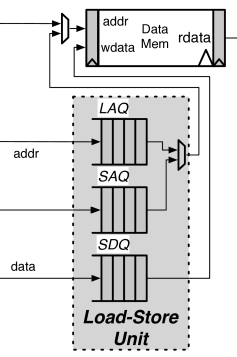
\includegraphics[angle=-90,width=0.5\linewidth]{boom_lsu_fig8_1}
			\bicaption{访存单元结构简化示意图。\citep{BOOMDoc2018}图8.1.}{Load-Store Unit simplified diagram. Figure 8.1 of \citep{BOOMDoc2018}.}
			\label{fig:LSU}
		\end{figure}
	\end{enumerate}

\section{研究方法与方案}
	纸上读来终觉浅,觉知此事要躬行。前面梳理了很多乱序多发射设计的相关工作与材料,最终还需要能转化为自己的设计。不过在设计之前,必须有一套开发验证的方法和平台,和一套成型的循序渐进由易到难的设计方案。这两个要素是开始设计必备的前提条件。
	
	\subsection{开发验证平台}
	
	本科学习期间采用的指令集是MIPS32,实验课上设计的单发射五级静态流水线处理器是基于龙芯提供的设计验证平台。设计中经历的步骤程序有:\textbf{step1}: 仿真时与龙芯提供的标准CPU loogson132生成(打印)的写回级trace对自动化的逐拍比对$ \Rightarrow $\textbf{step2}: 若比对出现不同则停止仿真,通过看波形找到产生不同写回信息的原因,并修正之$ \Rightarrow $如此循环往复直到仿真调通$ \Rightarrow $\textbf{step3}: 之后再用Vivado的集成化工具综合布局布线$ \Rightarrow $\textbf{step4}: 最后生成bitstream --- 可以配置FPGA的格式文件用JTAG线下载至Xilinx公司的FPGA上,产生物理上预期的效果就算设计完成。需要注意的是为了简化,课上实验中的内存是使用板卡上的SRAM模拟的,并不是真正的内存。
	
	但是这样一套自己比较熟悉的平台,却很难将RISC-V移植进来。没有现成的可以用来比对的标准trace;Chisel代码本身不支持波形调试,需要转化为低级的Verilog然后用仿真工具才能看波形,但是由Chisel转换而来的Verilog文件已经不是人可以阅读的形式了,有点像综合出来的网表格式。所以原来的平台并不奏效。
	
	很自然会想到在RISC-V开源处理器仓库中有没有可以略加修改便可使用的设计验证平台,于是尝试着阅读了Rocket和BOOM的说明文档及其代码。BOOM外围的很多代码是复用Rocket的,也就意味着存在着一种可能性 --- 区分出BOOM处理器自身和复用的Rocket代码,找到两者之间的接口,然后把BOOM替换为自主设计的处理器核心。但是不得不说,阅读代码的过程非常痛苦。首先BOOM和Rocket都已经是达到工业级别的颇为成熟的大工程了,里面的文件众多,每个文件中又有不同的类,而且这些类之间又有着非常复杂的交互关系。其次这些处理器的设计者和Chisel编译器的设计者属于一个团队,里面灵活使用到了Chisel和Scala中一些高级的语言特性来更为简洁,扩展性更强的描述电路,但是这些特性却是初学者一时很难理解的障碍。加之本设计的任务并不是在BOOM的基础上加些模块或者特性,也不是修改BOOM来达到性能的提高(再者说,这样难免有抄袭之嫌),任务在于自主设计出一款和BOOM一样完整的处理器的内核。所以如果需要和BOOM一样复用Rocket的外围代码,然后去跑仿真验证,就必须清楚的了解每一个细节,这一个熟悉的过程最少也需要几个月的时间,时间上来不及不允许。
	
	虽然BOOM和Rocket太过复杂驾驭不了,但是伯克利分校体系结构课程的教学用的是RISC-V,那么他们的实验就一定采用的是适合初学者的设计验证平台。果然,在伯克利分校CS152课程的网页上找到了他们实验平台,验证了这个思路是可行的。如今,这个实验的平台以及几个简单的能够在平台上运行的处理器核已经作为伯克利分校主要仓库目录列表ucb-bar中的\href{https://github.com/ucb-bar/riscv-sodor}{riscv-sodor仓库}开源了。同时还有一个\href{https://gitter.im/librecores/riscv-sodor}{论坛社区}(\url{https://gitter.im/librecores/riscv-sodor})。里面有很多初学者去提问,同时有包括RISC-V开发者在内的专家和热心的研究个体来答疑。所以对平台存在的疑问和漏洞都能在社区里提问,而经常浏览也能够学到很多初学者遇到的问题的原因以及背后的平台运行机制。其机制可以简化地用图\ref{fig:platform}来概括。
	\begin{figure}[!htbp]
		\centering
		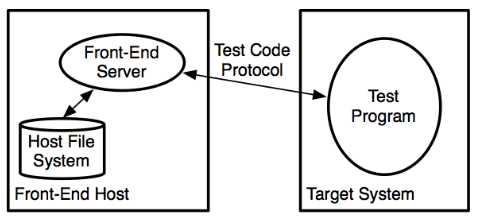
\includegraphics[width=0.5\linewidth]{platform}
		\bicaption{测试环境。前端服务器将RISC-V二进制文件加载到主机的文件系统中,启动目标系统的模拟器,发送RISC-V二进制代码到目标模拟器填充入模拟的处理器指令内存中。一旦前端服务器完成发送测试代码后,服务器重启目标处理器然后目标处理器就可以始从固定的地址开始执行程序。\citep{lab1}图2.}{The Testing Environment. The front-end server (fesvr) loads the RISC-V binary from the Host file system, starts the Target system simulator, and sends the RISC-V binary code to the Target simulator to populate the simulated processor’s instruction memory with the program. Once the fesvr finishes sending the test code, the fesvr resets the Target processor and the Target processor begins execution at a fixed address in the program. Figure 2 of \citep{lab1}.}
		\label{fig:platform}
	\end{figure}
	
	有了简单入门级的设计验证平台,再稍作修改,将原来糅杂在一个仓库中的处理器Chisel源代码和测试程序代码以及测试工具链如前端服务器软件和生成模拟器的C++库分离成两个相对独立的私有仓库,用git来管理,使得代码的编写工作变得更有条理。一级的文件目录结构如图\ref{fig:project}所示。同时,还对原来处理器源码的组织形式做了略微的调整,使得更符合JAVA的代码组织结构风格。另外,对于Makefile编译文件,也做了一些修改,使之符合自己的文件目录组织方式。
	\begin{figure}[!htbp]
		\centering
		\begin{subfigure}[b]{0.4\textwidth}
			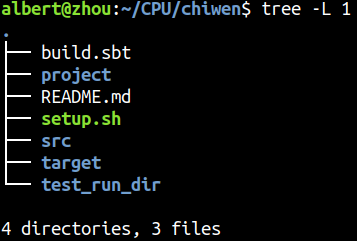
\includegraphics[width=\textwidth,height=4cm]{chiwen_L1}
			\caption{}
			\label{fig:chiwen_L1}
		\end{subfigure}\qquad%
		~%add desired spacing
		\begin{subfigure}[b]{0.4\textwidth}
			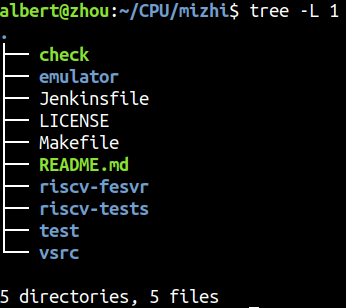
\includegraphics[width=\textwidth,height=4cm]{mizhi_L1}
			\caption{}
			\label{fig:mizhi_L1}
		\end{subfigure}
		\bicaption{毕业设计工程仓库。(a) 处理器Chisel源代码仓库。(b) 测试软件工具链和测试程序仓库。}{the repositories of the design. (a) The git repository which contains processors Chisel source, (b) The git repository which contains verification tool chain and test programs.}
		\label{fig:project}
	\end{figure}

	运行的流程大致为:
	\begin{itemize}
		\item 在\texttt{chiwen}目录下运行sbt,Scala的构建工具或者说是集成化的编译器(Chisel的编译器实际上是在sbt中加入前端的Chisel语法树分析,和后端的Chisel到Verilog的转化规则)。然后选择处理器的工程名,这样sbt就会产生一个处理器的C++精确到周期的描述。为了简化这一步骤,如图\ref{fig:chiwen_L1}编写了一个脚本,执行命令{\footnotesize \verb|terminal| -> \verb|./setup.sh processor_name|}即可。这个脚本最后会把生成的Verilog代码和Chisel的中间层表示Firrtl放到\texttt{mizhi}的\texttt{emulator}目录中以处理器名为目录名的目录下。
		\item 编译文件Makefile会用verilator软件将第一步得到的生成代码再生成和处理器对应的C++模拟器。
		\item 编译文件Makefile会调用RISC-V的前端服务器(fesvr)在文件系统中为第二步得到的C++二进制模拟器打开一个socket,然后将RISC-V的二进制文件文件传输到目标处理器去执行,见图\ref{fig:platform}.
		\item 在\texttt{mizhi}仓库里,已经提供了现成的测试程序包括指令功能测试和嵌入式benchmark程序性能测试(表\ref{tab:benchmark}列举了目前使用的八个程序),放在\texttt{riscv- tests}目录下。若要自己添加测试程序,可以放到test目录下,见图\ref{fig:mizhi_L1}. 程序的编译用RV32I的GCC工具链标准编译即可,这些具体的细节都掩藏在Makefile中,只需要输入命令{\footnotesize \verb|cd riscv-tests/isa| -> \verb|make|}生成指令测试二进制文件或者{\footnotesize \verb|cd riscv-tests/benchmarks| -> \verb|make|}生成性能测试的二进制文件。相应的,让目标处理器去仿真模拟执行只需要输入命令{\footnotesize \verb|make run-asm-tests|}或者{\footnotesize \verb|make run-bmarks-test|}就能运行指令功能测试或者benchmark性能测试。在Makefile中还提供了一些其他有用的命令。
		\item 最后如果通过,会在终端给出PASSED字样,否则就是FAILED来给出处理器的验证结果。大致的机理是Makefile会先用Spike,RISC-V的ISA级模拟器跑出一遍trace,然后比对处理器的输出结果。前端服务器(fesvr)也会通过debugIO通过访存来检测处理器的状态是否达到预期。不过存在着自动检测在FAILED时却给出PASSED的少见情况。针对这种情况,用python编写了一个脚本来比对待测试处理器产生的trace和Spike跑出的标准trace每一个周期的有效写回寄存器堆结果,或者也可以和sodor已经提供的几个简单处理器打印的trace做对比。这样就能严格保证处理器执行已有程序的正确性。
	\end{itemize}
	
	\subsection{设计方案}
	\begin{figure}[H]
		\centering
		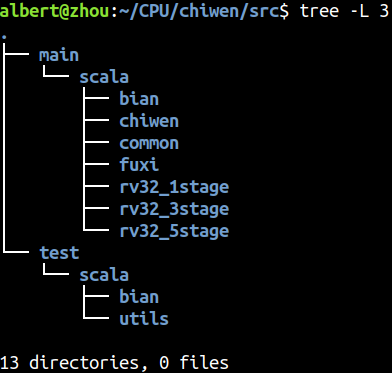
\includegraphics[width=0.4\linewidth]{chiwen_src_L3}
		\bicaption{目前为止已有的六款RISC-V RV32I处理器核。其中3款处理器CHIWEN(螭吻), FUXI, BIAN(狴犴)架构分别是自主设计的单发射五级静态流水线,双发射五级静态流水型, 和双发射乱序流水。另外3款rv32\_1stage, rv32\_3stage, rv32\_5stage是\href{https://github.com/ucb-bar/riscv-sodor}{riscv-sodor}提供的单周期、单发射三级静态流水线和单发射五级静态流水线处理器。common子目录包含了处理器共有的模块。}{The six Microprocessors based on RISC-V RV32I isa so far. There are three processors are self designed, including CHIWEN(single-issue, five-stage pipeline processor), FUXI(dual-isse, five-stage pipeline processor) and BIAN(two-wide superscalar processor with out-of-order). Other three simple processors are provided by \href{https://github.com/ucb-bar/riscv-sodor}{riscv-sodor}, with single cycle, three-stage and five stage single-issue architecture separately. \texttt{common} subdirectory contains common modules shared with all processors.}
		\label{fig:chiwen_src}
	\end{figure}

	若直接进行双发射乱序的设计,会因为没有很好的设计着力点而变得步履维艰。所以制定出一套详细的从易到难循序渐进的方案显得非常重要。同时,Chisel对于自己来说是一门全新的语言,也需要用一些简单的任务来充分地熟悉。
	
	在riscv-sodor中已经提供的有三款简单的处理器,分别是单周期(rv32\_1stage)、单发射三级静态流水线(rv32\_1stage)和单发射五级静态流水线(rv32\_5stage)。将它们拷贝至自己的仓库的文代码目录中,参见图\ref{fig:chiwen_src}。这些简单的处理器除去CSR特权寄存器逻辑的设计之外,处理器核心仅仅只有500多行代码,代码非常简洁易读,尤其是其译码部分。处理器采用的结构是经典的数据通路和指令通路。但是事实上这样的设计模式不好,两个通路之间是强耦合的。在阅读rv32\_5stage的过程中,也发现数据通路和控制通路的两个文件中相当有一部分代码是重复冗余的。为了可拓展性和控制复杂性的考虑,第一步是调整处理器的设计模式,采用和BOOM一致的前后端模式。重新对单发射五级流水修改后版本成为了处理器CHIWEN。同时,在修改的过程中,逐渐掌握了Chisel描述电路的常用写法。
		
	\begin{table}[!htbp]
		\bicaption{benchmark性能测试程序说明。除了coremark是自己添加的,其余的都是\href{https://github.com/riscv/riscv-tests}{riscv-tests}已经提供的}{The explanation of the set of benchmarks provided by the  \href{https://github.com/riscv/riscv-tests}{riscv-tests} repository except for coremark}
		\label{tab:benchmark}
		\centering
		\footnotesize% fontsize
		\setlength{\tabcolsep}{4pt}% column separation
		\renewcommand{\arraystretch}{1.2}%row space 
		\begin{tabular}{lcc}
			\hline
			名称 & 功能解释 & 备注 \\%inserts table 
			%\cline{2-9}% partial hline from column i to column j
			\hline
			coremark    & A synthetic embedded integer benchmark      & 合成的嵌入式整数程序 \\
			dhrystone   & A synthetic embedded integer benchmark.     & 合成的嵌入式整数程序 \\
			median 		& Performs a 1D three element median filter.  & 一维的中位数查找 \\
			multiply 	& A software implementation of multiply.      & 乘法的软件实现 \\
			qsort  		& Sorts an array of integers using quick sort. & 快速排序 \\
			rsort  		& Sorts an array of integers using radix sort. & 基数排序 \\
			towers 		& Solves the Towers of Hanoi puzzle recursively. & 汉诺塔 \\
			vvadd 		& Sums two arrays and writes into a third array. & 数组向量加法 \\
			\hline
		\end{tabular}
	\end{table}

	但是CHIWEN不是对rv32\_5stage简单重写。事实上rv32\_5stage运行benchmark(见表\ref{tab:benchmark})的统计结果显示,IPC普遍偏低。%TODO: add figures
	原因在于rv32\_5stage更没有转移猜测的机制,如果跳转指令的结果还没计算出来,就顺序往后取指。RISC-V没有延迟槽,而且在第三级计算出跳转目标和方向只有还会锁存一个周期再进入取指部件重定向取指。所以猜错一个分支跳转指令就会损失2个周期,这样IPC就不会高。所以第二个任务就是在CHIWEN的前端加入转移预测器,参考借鉴的是\citet{Celio:EECS-2017-157}中的BTB,BPD和RAS设计,做了一定简化。
	
	在riscv-sodor平台上取指和访存都是没有延迟的,默认是同步的逻辑。为了模拟真实的外围内存系统,写了一个带有随机性的延迟的中间桥放在处理器核和模拟的同步内存之间,并且采用的是AXI的标准接口。接着构建了容量为16KB的icache来缓存指令,提高在有延迟的取指环境中的处理器性能。但是出于简化设计的考虑,并没有构建dcache,访存没有延迟,为默认的同步时序。综上,前后端的模式的五级流水线架构,辅以转移预测器和icache构成了CHIWEN处理器。
	
	前后端模式的强大优势在于,从单发射的CHIWEN过渡到超标量宽度为2的双发射五级静态流水线FUXI的过程非常平稳,代码基本上能够复用,不用做大的修改,开发的时间和调试的时间都大大缩短了。
	\begin{itemize}
		\item 后端的修改较为简单,把CHIWEN的后端用Chisel里Vec的写法重新写一遍,构建出两条并行的后端执行流水线。然后解决两条并行指令之间的如写后写、写后读、同时为跳转指令、同时为访存指令、同时为特权态指令等冲突,将后一条指令停住一个周期做成串行执行。不光写起来简单,调试的时候也不会出现很多的bug。
		\item 前端的修改是重点,也是难点,涉及到icache和分支预测器都会做出调整修改。在后面设计实现的章节中做具体的介绍。
	\end{itemize}
	
	有了CHIWEN和FUXI这两代处理器核微结构的演进,然后才真正过渡到双发射乱序处理器BIAN的设计调试中。由于FUXI和BIAN都是超标量宽度为2的处理器,所以BIAN的前端可以完全复用FUXI的,而不需要单独重新设计。解决了前端的问题,最后就可以集中力量进行后端乱序发射的逻辑设计,前后端强大的优势再次得到了很好的体现。而且可以看的出来,最后高性能双发射乱序处理器的设计成功离不开由易到难循序渐进的正确设计路线。
	
	\subsection{调试手段}
	
	首先是模块级的调试验证。Verilog常用的做法是给待测模块写激励测试。这个激励测试相当于更大一级的测试激励模块,里面实例化了待测模块并构建有时钟时序和测试输入,然后通过仿真器人眼查看输出信号波形是否符合预期。如果真的编写过Verilog激励模块,就会真切的体会到编写过程的麻烦,不仅是因为语句的粒度太小,而且就算波形出现和预期不同的结果,也不能马上下待测模块有漏洞的结论,因为可能是激励模块写得有漏洞。在这样的背景下,Chisel语言自封闭的设计了一套基于Chisel和Scala编写模块验证的方式。它封装了\texttt{chisel3.iotesters.PeekPokeTester}的基类,编写待测模块的激励模块首先继承这个基类,待测模块输入端的赋值调用poke语句,输出端的验证可以用expect语句和预期值进行自动比对,也可以打印出来。同时,因为Scala是脚本语言,所以复杂的且带随机性的激励测试构造是便捷的。另外,最为关键的一点是,\texttt{chisel3.iotesters.PeekPokeTester}基类隐藏了时序的构造,因为电路的何时复位,时钟的频率多少,何时在上升沿对电路功能的仿真几乎没有影响。电路经过一个时钟周期的逻辑在Chisel的测试代码中用简单的\texttt{step(1)}就可以实现(括号中的1表示一个周期)。在\texttt{step(1)}之后的代码逻辑就会发生在\texttt{step(1)}之前代码逻辑的一个周期之后。Chisel的测试代码的组织形式和JAVA保持一致,见图\ref{fig:chiwen_src}中的test目录,这样方便管理和测试,特别是在IDE的编辑环境中。
	
	但是上述调试方法不再适用于将各个模块整合起来的整个系统。整个系统的激励输入还是要依赖于riscv-sodor的测试环境(见图\ref{fig:platform})。那么输出端又如何去验证呢?首先分析输出端核心的信号有哪些,最核心的是每一周期的寄存器堆写回信息加上store指令的内存写回的信息。如果这两方面的信息都符合预期就认为处理器的输出是正确的。这个预期可以由RISC-V的模拟器Spike得到的,也可以由经过验证的开源的处理器核如rv32\_5stage来得到。调试的流程为:\textbf{step1}: 写回信息打印出来以文本的形式存储$ \Rightarrow $\textbf{step2}: 用自己编写的一个自动对比的python脚本进行文本操作自动比对$ \Rightarrow $\textbf{step3}: 定位到开始出现不同的第一个周期$ \Rightarrow $\textbf{step4}: 在源代码中加入在这个周期之前一个窗口内打印与产生差错有关联的更多变量的代码$ \Rightarrow $\textbf{step5}: 重新编译执行$ \Rightarrow $\textbf{step6}: 通过分析文本中的调试信息来定位到源代码中的bug。
	
	这样调试方式虽然原始,如果需要重新加入打印信号,就需要重新编译执行。但是就其速度而言,因为不用做整个系统全信号的仿真模拟,仅仅是打印出是每一周期的写回信息以及一段窗口内的详细的相关变量信号而已,就算加上重新编译和执行的时间,也比波形图仿真更快。另外,由于设计的时候先采用了较为彻底的模块级验证,等到整合为完整系统时,bug数量大大降低了,而且基本集中在各个模块交互的逻辑上。同时,文本的优势在于可以灵活地编写一些文本操作的脚本做自动化的分析,这恰恰是波形所不具备的。比如需要得到某一周期执行级具体的指令,波形图上只能显示一个32位的数值,转化需要人工手动。但是文本就可以用一个脚本来自动转化。还有例如分析分支跳转预测正确率的过程中需要统计精确到不同跳转指令的误预测率时或者某一周期窗口内的跳转行为以及预测行为时,文本+脚本分析的手段都要明显优于波形图调试。
	
	正是采用了这种调试手段,从最开始的调试方式摸索阶段,用两周时间调通了带转移预测器的CHIWEN处理器,并且预测器的行为符合预期;再到用一周时间调通FUXI的前端,加上三天调通FUXI的后端;最后到用两周的时间(一周进行模块级的调试验证,一周进行整合系统的调试验证)调通了整合到FUXI前端的BIAN的后端。调试的时间的减少使得在微结构的设计上的时间变得相对充裕。